%%==================================================================%%
%% Author : Tejedo Gonz�lez, Daniel                                 %%
%%          S�nchez Barreiro, Pablo                                 %%
%% Version: 1.0, 18/11/2012                                         %%                   %%                                                                  %%
%% Memoria del Proyecto Fin de Carrera                              %%
%% Antecedentes, archivo ra�z                                       %%
%%==================================================================%%

\chapterheader{Antecedentes}{Antecedentes}
\label{chap:background}

Este cap�tulo trata de describir a grandes rasgos las t�cnicas, tecnolog�as y herramientas utilizadas para la creaci�n de nuestro entorno de especificaci�n y validaci�n de restricciones. El cap�tulo comienza describiendo m�s en detalle lo que es la Ingenier�a de Lenguajes Dirigida Por Modelos, para a continuaci�n presentar las dos principales herramientas de modelaci�n que han sido utilizadas: Ecore y EMFText. M�s adelante se hablar� tambi�n en detalle de los �rboles de caracter�sticas, y por �ltimo se describir� brevemente el entorno de desarrollos de plugins de Eclipse que se utiliz� para implementar diversas funciones de nuestro editor.

\chaptertoc

\section{Ingenier�a de Lenguajes Dirigida por Modelos}
\label{sec:back:ildm}
%%==================================================================%%
%% Author : Tejedo Gonz�lez, Daniel                                 %%
%%          S�nchez Barreiro, Pablo                                 %%
%% Version: 1.0, 18/11/2012                                         %%                   %%                                                                  %%
%% Memoria del Proyecto Fin de Carrera                              %%
%% Antecedentes, Ingenier�a de lenguajes dirigidos por modelos                            %%
%%==================================================================%%

La Ingenier�a de Lenguajes Dirigida por Modelos no es m�s que un caso concreto de la m�s gen�rica Ingenier�a Dirigida por Modelos (o Model-Driven Architecture o MDA) aplicado desde el punto de vista de la Teor�a de Lenguajes Formales, con lo cual es conveniente explicar en qu� consiste MDA y comentar los a�adidos que introduce el enfoque gram�tico.

La Inginier�a Dirigida por Modelos intenta definir la funcionalidad de el sistema que pretendemos crear a trav�s de la creaci�n de uno o varios metamodelos que representen todas las caracter�sticas de nuestro sistema y todas las operaciones que puede llevar a cabo. El principal objetivo de la Ingenier�a Dirigida por Modelos es elevar el nivel de abstracci�n a�n m�s, situ�ndolo por encima del l�mite establecido por los Lenguajes de Alto Nivel. 

El nivel de abstracci�n y complejidad de nuestros metamodelos variar� dependiendo de la cantidad de ellos que incorporemos al sistema. De este modo, un metamodelo que represente todo el sistema directamente ser� m�s dif�cil de entender a primera vista que varios metamodelos que implementen cada uno un tipo de operaci�n o funcionalidad del sistema.

La transformaci�n de esos modelos a c�digo permite la automatizaci�n de tareas que pueden resultar triviales y/o repetitivas al programador, en las cuales de otro modo se invierte mucho tiempo de programaci�n y de detecci�n y depuraci�n de errores. 

Una vez que tengamos los metamodelos necesarios para definir el comportamiento de nuestro sistema, podremos instanciarlos para crear modelos que representen sistemas concretos. Una instancia de un metamodelo es un modelo que cumple todos los requisitos marcados por su metamodelo, y que da valor a los par�metros del mismo (por ejemplo a sus atributos).

La figura \ref{fig1} es un ejemplo de un metamodelo sencillo que represente un constructor de grafos unidireccionales con pesos. O dicho de otro modo, representa la sintaxis abstracta de nuestro sistema. Se denomina modelo de sintaxis abstracta a cualquier metamodelo que represente los conceptos y el comportamiento del sistema, y cuyas instancias representen elementos reconocibles dentro de ese sistema.

\begin{figure}[t]
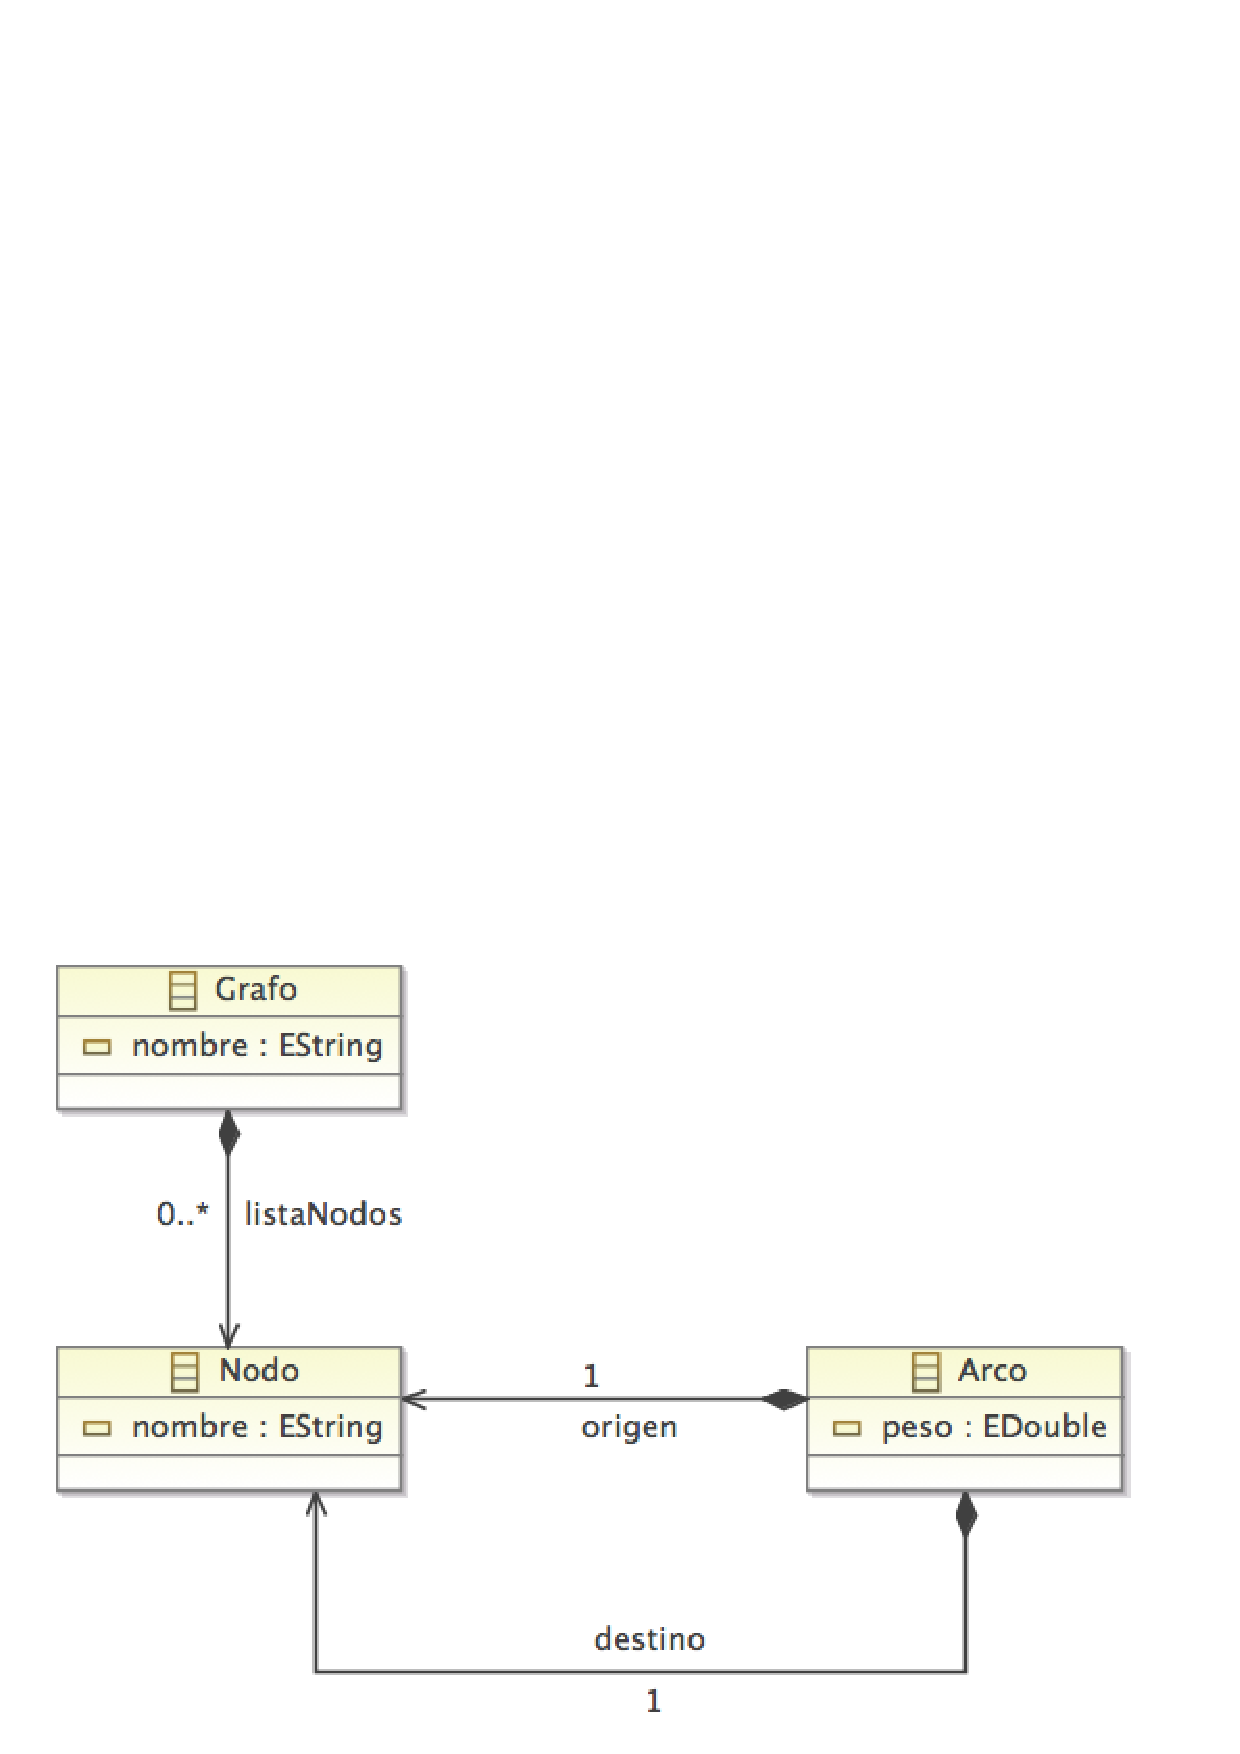
\includegraphics[scale=0.5]{background/abstracta.jpg}
\caption{Metamodelo (sintaxis abstracta) de un creador de grafos}
\label{fig1}
\end{figure}

En el ejemplo presentado, el metamodelo presenta la sintaxis abstracta de nuestro sisstema porque cualquier instanciaci�n v�lida del mismo constituye un grafo completo. Dentro del contexto particular de la Ingenier�a de Lenguajes Dirigida por Modelos, la sintaxis abstracta representa cualquier conjunto de l�neas de c�digo v�lidas que pueden construirse a partir de ella, y posteriormente ser ejecutadas.

Explicando el metamodelo de nuestro ejemplo un poco m�s en detalle, podemos decir que la clase Grafo representa el conjunto final de un grafo construido, y puede tener varios Nodos. Esos nodos, a su vez, pueden estar conectados por Arcos. Cada arco tiene un origen, un destino y un peso. Cualquier instanciaci�n de este metamodelo representa un grafo completo.

La figura \ref{fig2} muestra un ejemplo de instanciaci�n del metamodelo anterior. Esta instancia representa un grafo sencillo que muestra las distancias entre algunas ciudades. O dicho de otro modo, es una de las m�ltiples sintaxis concretas que podemos construir a partir de nuestra sintaxis abstracta. 

\begin{figure}[t]
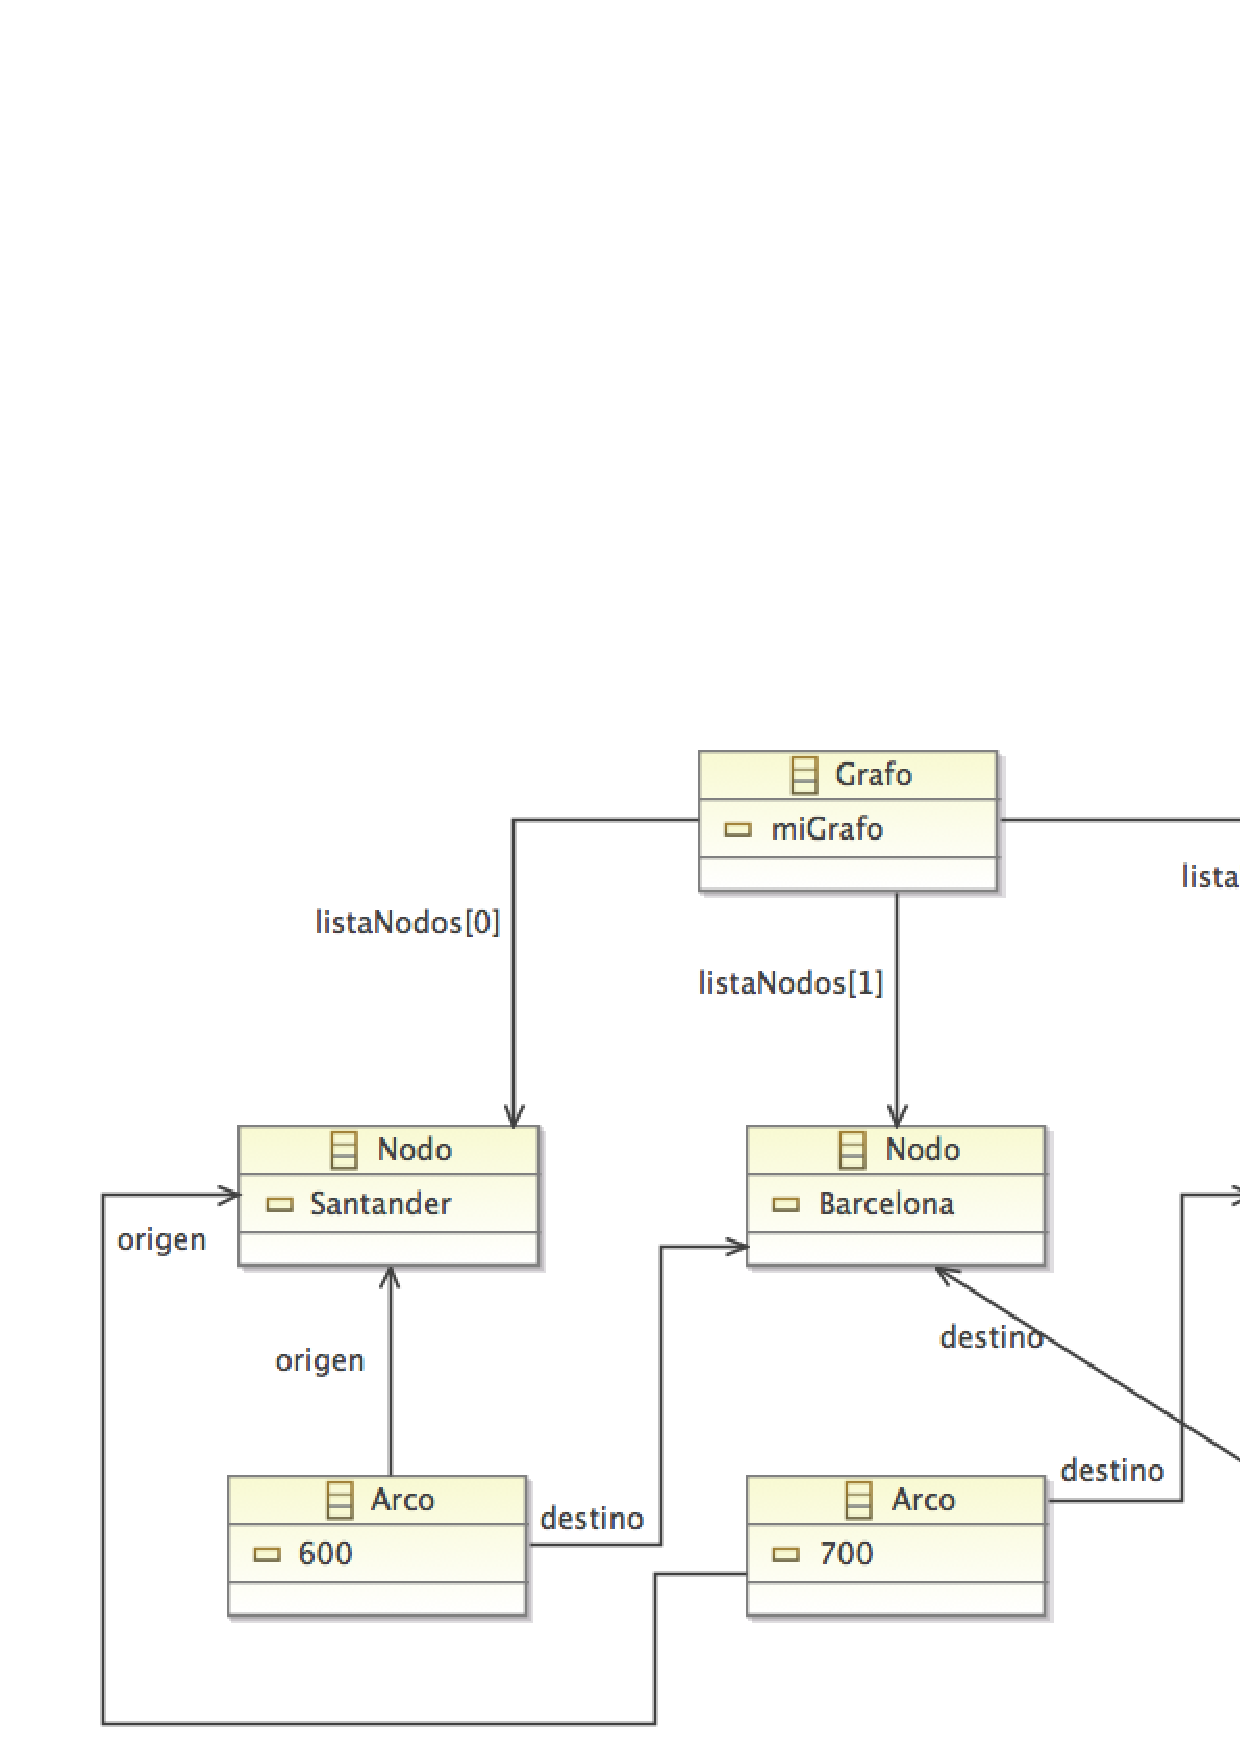
\includegraphics[scale=0.5]{background/concreta.jpg}
\caption{Instancia del metamodelo (sintaxis concreta) que representa un grafo espec�fico}
\label{fig2}
\end{figure}

Dentro del marco de la Ingenier�a de Lenguajes Dirigida por Modelos, una sintaxis concreta es cualquier conjunto de expresiones v�lidas que hayan sido generadas con nuestra sintaxis abstracta. Pero no s�lo eso, el hecho de que estemos trabajando con lenguajes conlleva irrevocablemente el tener que desarrollar una gram�tica de producciones para poder construir nuestras l�neas de c�digo en el orden apropiado y con los s�mbolos apropiados. Eso s�, la gram�tica ser� m�s sencilla y comprensible que la que habr�a que construir de no estar usando este tipo de metodolog�a. Esta tarea tambi�n queda englobada en la sintaxis concreta. De este modo, la sintaxis concreta se suele clasificar en sintaxis concreta visual (el modelo, expresado mediante l�neas de c�digo en el caso de lenguajes, o un grafo pintado en el caso del ejemplo mostrado) y sintaxis concreta textual (la gram�tica del lenguaje).

La figura \ref{fig3} muestra una sintaxis concreta visual del grafo de la figura \ref{fig2}.

\begin{figure}[t]
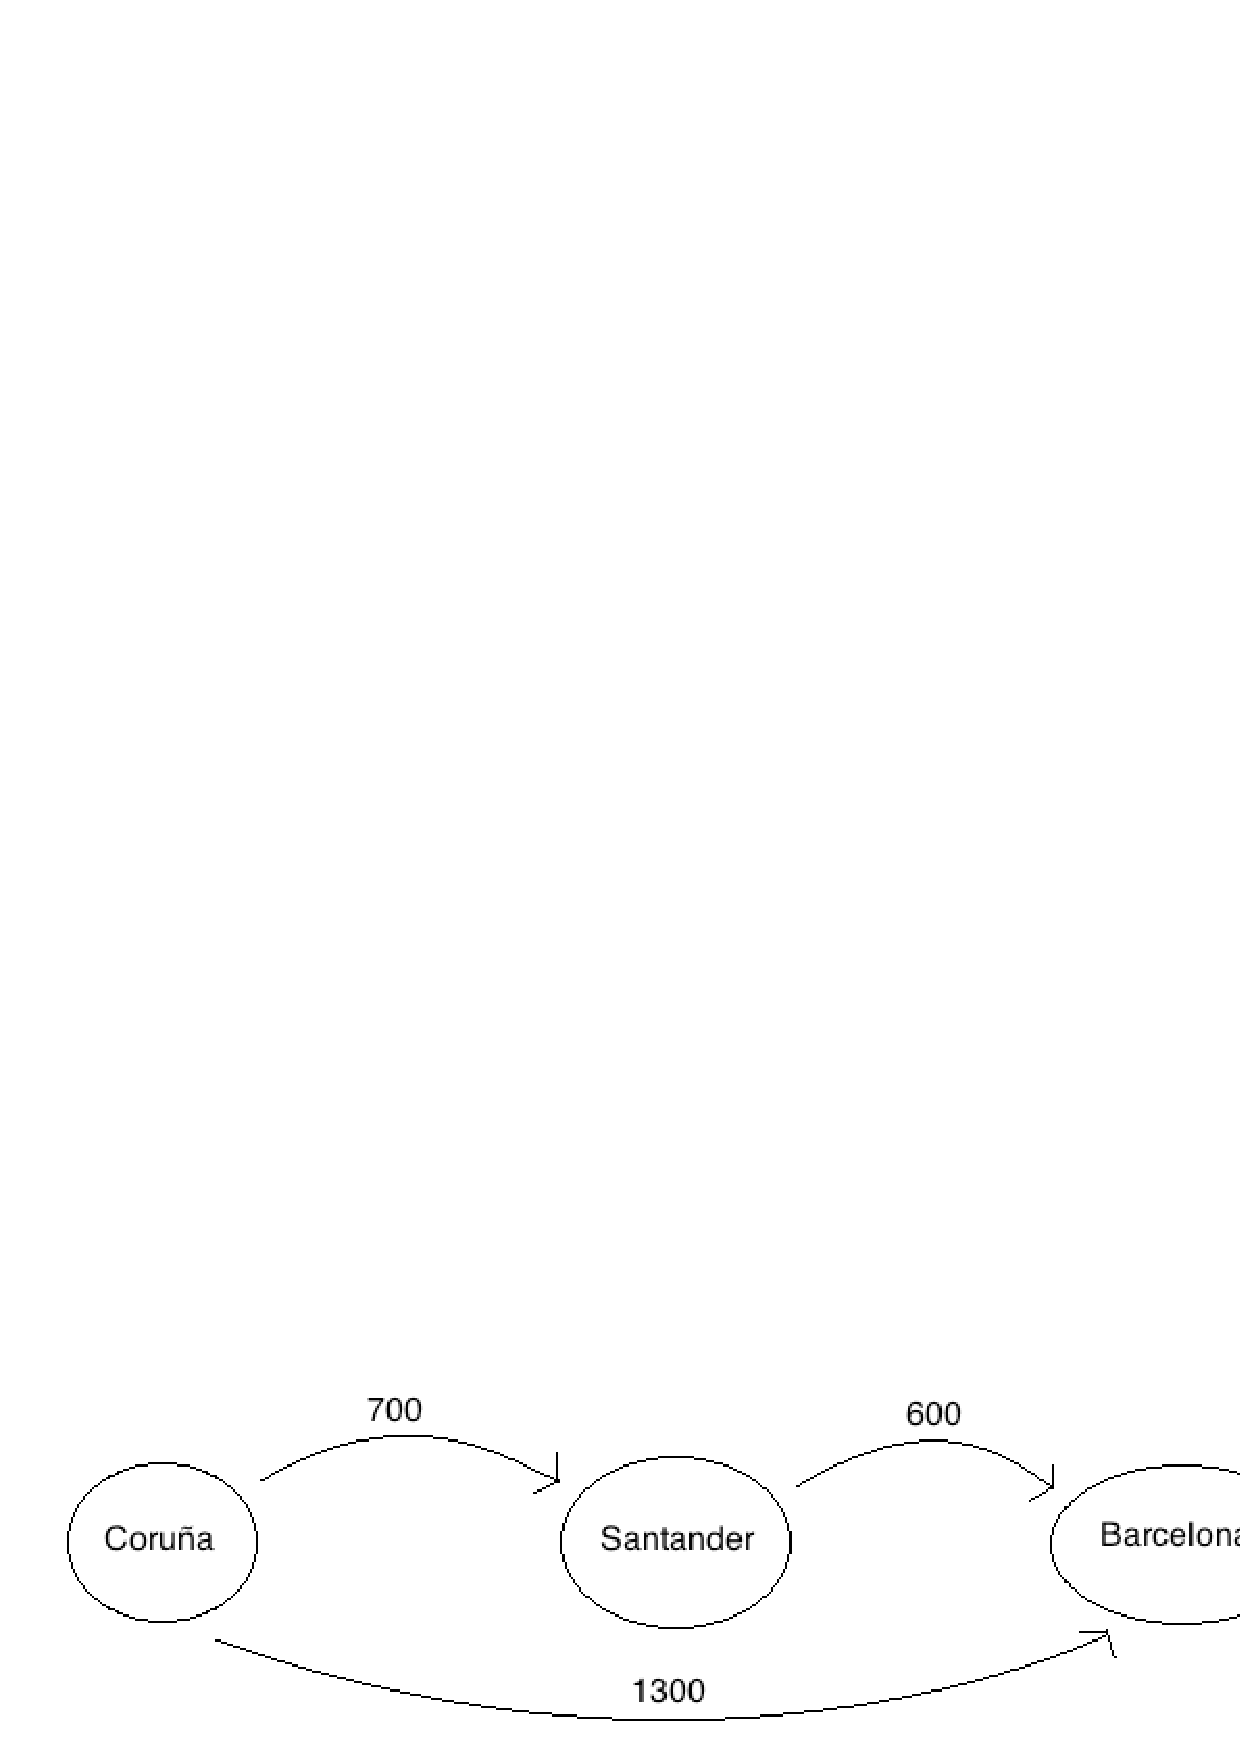
\includegraphics[scale=0.5]{background/grafo.jpg}
\caption{Sintaxis visual del grafo de la figura \ref{fig2}}
\label{fig3}
\end{figure}

Una vez que hemos completado estos pasos, s�lamente queda dotar al sistema de una sem�ntica, es decir, de un comportamiento en ejecuci�n. En el ejemplo de nuestro generador de grafos podr�amos crear una sem�ntica para calcular distancias m�nimas entre caminos. En el caso concreto de la Ingenier�a de Lenguajes Dirigida por Modelos esta sem�ntica representa el comportamiento de las l�neas de c�digo cuando son ejecutadas. Por poner un ejemplo sencillo, es la encargada de que la instrucci�n "4 < 5" compruebe si efectivamente el 4 es menor que el 5.

Una vez se han explicado las bases de la Ingenier�a de Lenguajes Dirigida por Modelos vamos a proceder a mostrar y explicar muy brevemente el metamodelo usado para generar las estructuras v�lidas de c�digo para el lenguaje de especificaci�n y validaci�n de restricciones que hemos creado en este PFC. Ese metamodelo corresponde a la figura \ref{fig4}

\begin{figure}[t]
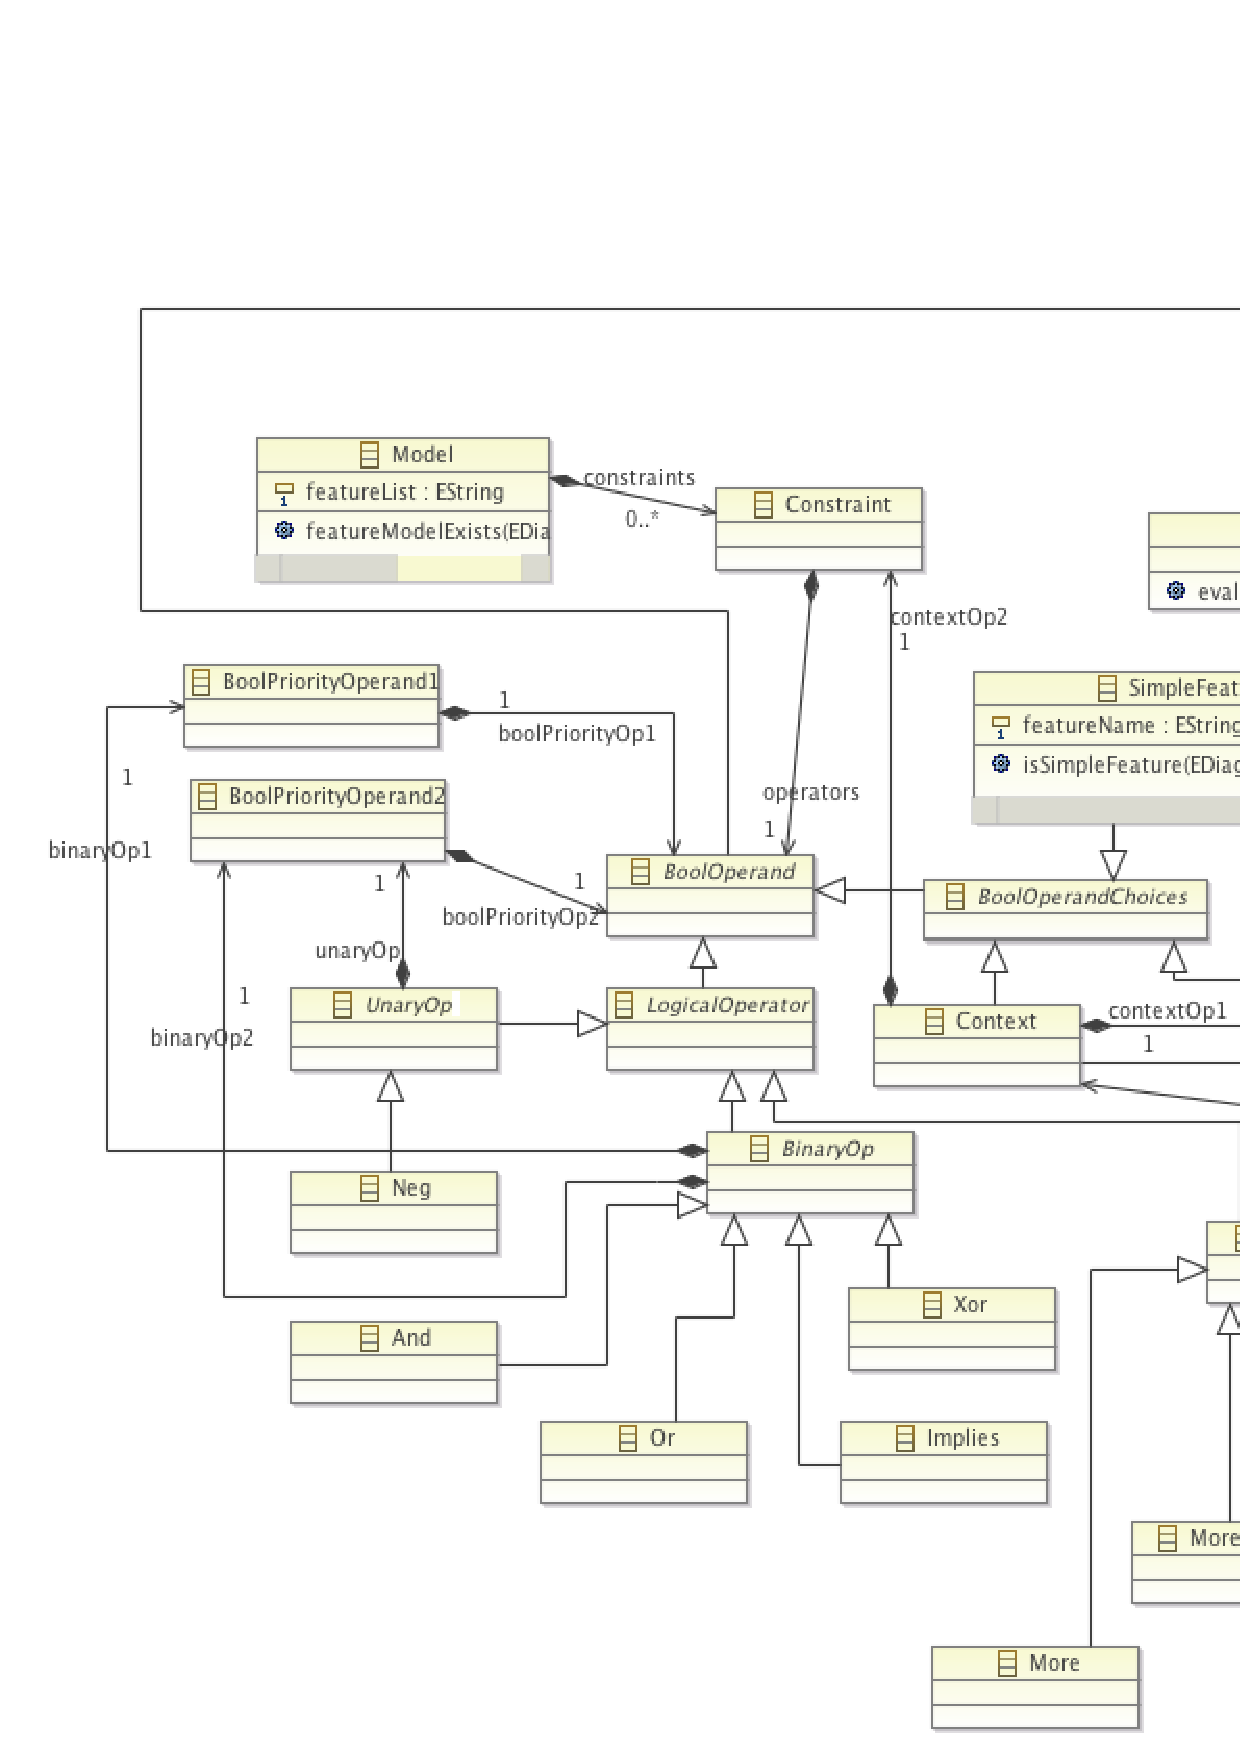
\includegraphics[scale=0.4]{background/metamodelo.jpg}
\caption{Metamodelo utilizado para la creaci�n de nuestro lenguaje de especificaci�n y validaci�n de restricciones}
\label{fig4}
\end{figure}

La clase que engloba todo el conjunto resultante es Model. Un modelo puede tener varias restricciones, y estas a su vez pueden tener varias operaciones booleanas (ya que una restricci�n siempre tiene que evaluarse a true o false). Esas operaciones booleanas se dividen en varios tipos: unarias (negaci�n) , binarias (and, or, etc.), de comparaci�n ( mayor que, menor que, etc.). o de selecci�n (all, any)  Los operandos pueden ser otras operaciones o caracter�sticas (en ingl�s Features). M�s adelante se explicar� en detalle la sintaxis del lenguaje creado.









 

\section{EMF, Ecore y EMF Validation Framework}
\label{sec:back:ecore}
%%==================================================================%%
%% Author : Tejedo Gonz�lez, Daniel                                 %%
%%          S�nchez Barreiro, Pablo                                 %%
%% Version: 1.0, 18/11/2012                                         %%                  
%%                                                                  %%
%% Memoria del Proyecto Fin de Carrera                              %%
%% Antecedentes, ecore                                              %%
%%==================================================================%%

EMF \emph{Eclipse Modeling Framework}~\cite{steinberg:2008} es un \emph{plug-in} para Eclipse~\cite{clayberg:2008} que permite elaborar metamodelos. Pera ello proporciona un lenguaje de metamodelado denominado Ecore, el cual se ha convertido en el est�ndar \emph{de facto} para la realizaci�n de metamodelos. Utilizando Ecore se pueden crear metamodelos de forma gr�fica usando una notaci�n muy similar a la los diagramas de clases de UML. La Figura~\ref{fig:sle:metamodeloGrafo} muestra un sencillo ejemplo de metamodelo en Ecore (ver Secci�n~\ref{sec:intr:sle} para m�s detalles). EMF tambi�n incorpora una herramienta para la validaci�n reglas adicionales que no puedan ser especificadas a nivel de del metamodelo. 
 
EMF permite que, a partir de un metamodelo especificado en Ecore, podamos, utilizando diversos generadores de c�digo, crear autom�ticamente un conjunto de clases que nos permiten manipular dichos modelos a nivel de c�digo. Dichas clases se pueden adem�s distribuir como \emph{plug-in} para el entorno Eclipse.

Adem�s, al haberse convertido en est�ndar \emph{de facto} para el desarrollo de metamodelos, Ecore es compatible con multitud de herramientas para Ingenier�a de Lenguajes Dirigida por Modelos, como EMFText, la cual se describe en la siguiente secci�n, o diversos generadores de c�digo o herramientas de transformaci�n de modelos. 



\section{EMFText}
\label{sec:back:emftext}
%%==================================================================%%
%% Author : Tejedo Gonz�lez, Daniel                                 %%
%%          S�nchez Barreiro, Pablo                                 %%
%% Version: 1.0, 18/11/2012                                         %%
%% Version: 2.0, 06/02/2013                                         %%
%%                                                                  %%
%% Memoria del Proyecto Fin de Carrera                              %%
%% Antecedentes, emftext                                            %%
%%==================================================================%%


EMFText~\cite{emftext:2009} es una herramienta para dise�ar sintaxis textuales para metamodelos Ecore, siguiendo un enfoque de Ingenier�a de Lenguajes Dirigida por Modelos. Utilizando EMFText podemos definir la sintaxis textual de un lenguaje software utilizando una notaci�n similar a las de las notaci�n BNF. La Figura~\ref{fig:sle:gramaticaGrafos} muestra un ejemplo de gram�tica definida en EMFText para el lenguaje de grafos presentado en la Secci�n~\ref{sec:intr:sle}. 

%%==================================================================%%
%% NOTA(Pablo): Aqu� haz una gram�tica en EMFText para el lenguaje  %%
%%              de grafos del Cap�tulo 1                            %%
%%==================================================================%%

\begin{figure}[!tb]
    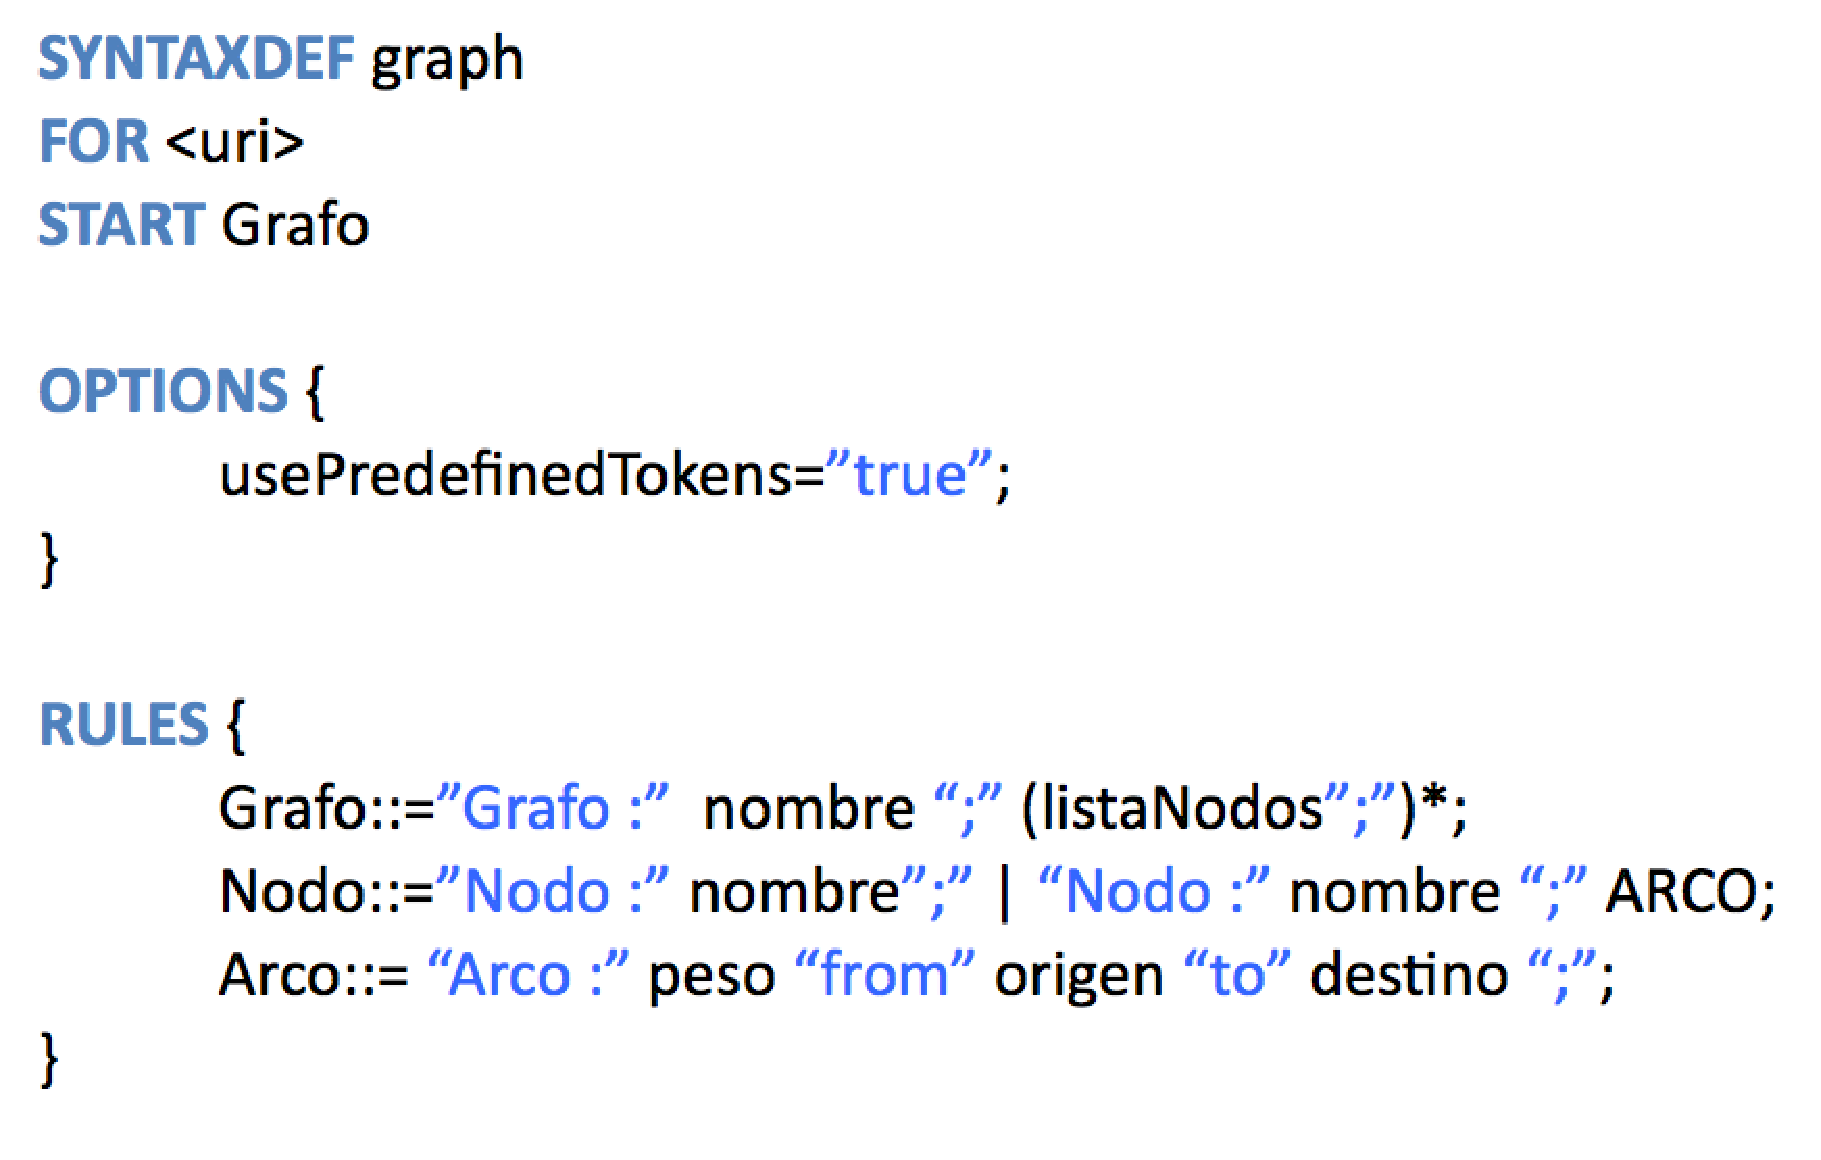
\includegraphics[scale=0.25]{background/gramaticaGrafo.eps}
    \caption{Gram�tica para el ejemplo del lenguaje de los grafos}
    \label{fig:sle:gramaticaGrafos}
\end{figure}

La sintaxis de EMFText difiere de las sintaxis BNF en que existen una serie de directivas para asociar elementos de la sintaxis textual con metaclases, de forma que se generen instancias de dichas metaclases a medida que se procesa el c�digo de un modelo. Por ejemplo, tal y como est� definida la gram�tica de la Figura~\ref{fig:sle:gramaticaGrafos}, a medida que vamos definiendo los arcos estamos indicando la informaci�n tanto de su peso como de sus nodos origen y destino. De este modo, EMFText genera una instanciaci�n de la metaclase Arco que inicializa con los datos le�dos y la a�ade a la instancia global del metamodelo.

La gran ventaja de EMFText es permite generar, a partir de la definici�n de una gram�tica, una gran cantidad de c�digo, liberando al programador de tareas tediosas que adem�s en muchos casos podr�an resultar complicadas. Utilizando EMFText se puede generar autom�ticamente: (1) un editor para nuestro lenguaje, con facilidades como coloreado de la sintaxis o autocompletado; (2) un procesador para el lenguaje capaz de generar una instancia de su correspondiente metamodelo; y (3) el c�digo necesario para empaquetar y distribuir dicho editor como un \emph{plug-in} para Eclipse. Adem�s, todo el c�digo generado es completamente independiente de EMFText, por lo que puede ser ejecutado en plataformas que no tengan instalado dicha herramienta; y es personalizable. Por ejemplo, se puede modificar f�cilmente el postprocesador de nuestra gram�tica. 






\section{�rboles de caracter�sticas}
\label{sec:back:fmodels}
%%==================================================================%%
%% Author : Tejedo Gonz�lez, Daniel                                 %%
%%          S�nchez Barreiro, Pablo                                 %%
%% Version: 1.0, 18/11/2012                                         %%                   %%                                                                  %%
%% Memoria del Proyecto Fin de Carrera                              %%
%% Antecedentes, �rboles de caracter�sticas                                    %%
%%==================================================================%%

El objetivo de las l�neas de productos software es crear la infraestructura para la r�pida  producci�n de sistemas software para un segmento de mercado espec�fico, donde estos sistemas software son similares, y aunque comparten un subconjunto de caracter�sticas comunes, tambi�n presentan variaciones entre ellos ~\ref{} ~\ref{} ~\ref{} ~\ref{}.

El principal logro en las l�neas de productos software es, construir productos espec�ficos lo m�s autom�ticamente posible a partir de un conjunto de elecciones y decisiones adoptadas sobre un modelo com�n, conocido como modelo de referencia, que representa la familia completa de productos que la l�nea de productos software cubre.

El desarrollo de l�neas de producto software se compone de dos procesos de desarrollo software diferentes pero �ntimamente relacionados, conocidos como ingenier�a del dominio e ingenier�a de la aplicaci�n.

En el nivel de ingenier�a del dominio, comenzamos por los documentos de requisitos que describen una familia de productos similares para un segmento de mercado espec�fico. Entonces, dise�amos una arquitectura e implementaci�n de referencia para esta familia de productos. Esta arquitectura de referencia contiene los elementos que son comunes para todos los productos de la familia.

En el nivel de ingenier�a de la aplicaci�n, comenzamos un documento de requisitos de un producto espec�fico. Este documento estable las variaciones espec�ficas que deben ser incluidas en este producto concreto. Con esta informaci�n, introducimos los cambios en la arquitectura y en la implementaci�n de referencia, y se deber�a obtener como resultado un producto software �nico.

Para ser capaces de completar con �xito la tarea correspondiente a ingenier�a del dominio, una de las cuestiones clave es establecer una forma de especificar los productos software que una l�nea de productos es capaz de productor, y aqu� es donde entran en juego los �rboles de caracter�sticas o Modelos de Caracter�sticas. Los productos de una l�nea de productos software se diferencian por sus caracter�sticas, siendo una caracter�stica un incremento en la funcionalidad del producto, o m�s formalmente, "una caracter�stica es una propiedad de un sistema que es relevante a algunos stakeholders y es usada para capturar propiedades comunes o diferenciar entre sistemas de una misma familia" ~\ref{}. De este modo un producto queda representado por las caracter�sticas que posee. 

Para poder capturar las divergencias y caracter�sticas comunes entre los distintos productos, los modelos de caracter�sticas organizan el conjunto de caracter�sticas jer�rquicamente mediante las siguientes relaciones entre ellos: (1) relaci�n entre una o varias caracter�sticas padre y un conjunto de caracter�sticas hijas o subcaracter�sticas y (2) relaciones no jer�rquicas del tipo "si la caracter�stica A aparece, entonces la B se debe excluir".

Por otro lado, un modelo de caracter�sticas debe poder representar la cardinalidad de las caracter�sticas, por motivos tanto de comprensi�n (es mucho mejor contar con un �rbol de 8 nodos que con uno de 100, teniendo ambos un significado equivalente), como de funcionalidad, ya que permite expresar ciertas restricciones que de no contar con la cardinalidad no podr�an expresarse. 

Las posibles relaciones que pueden darse en un �rbol de caracter�sticas (mostradas gr�ficamente en la figura \ref{fig6}) son las siguientes:

\begin{figure}[t]
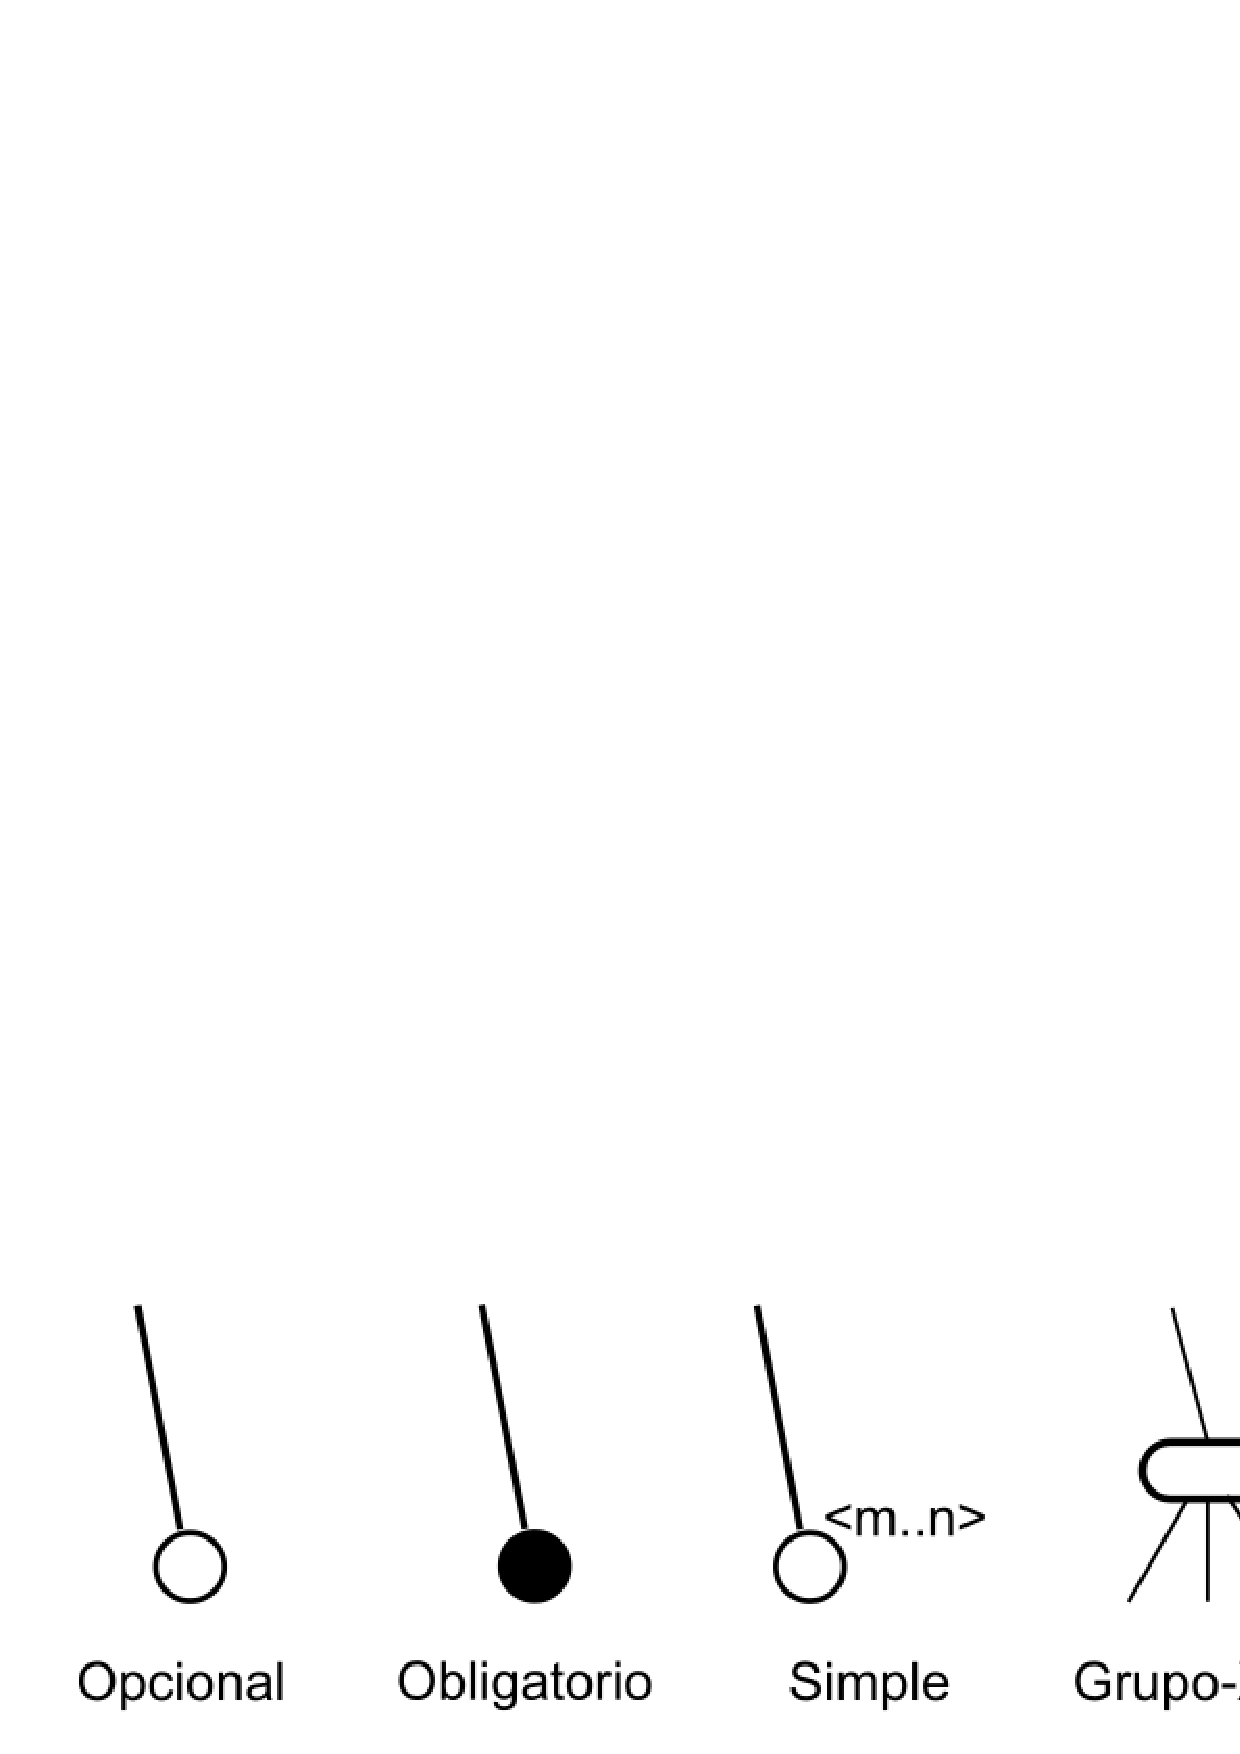
\includegraphics[scale=0.35]{background/relations.jpg}
\caption{Distintos tipos de relaciones en un modelo de caracter�sticas }
\label{fig6}
\end{figure}

1 - Opcional: La caracter�stica hija puede estar o no estar seleccionada
2 - Obligatoria: La caracter�stica es requerida.
3 - Simple: La caracter�stica tendr� una cardinalidad <m,n>, siendo m y n n�meros enteros que denotan el m�nimo y el m�ximo respectivamente de caracter�sticas que podemos seleccionar.
4 - Grupo-xor: S�lo una de las caracter�sticas pertenecientes al grupo ser� seleccionada.
5 - Grupo-or: Podremos seleccionar como m�nimo una de las subcaracter�sticas, y como m�ximo todas.
6 - Grupo simple: El n�mero de caracter�sticas seleccionadas del grupo vendr� dado por su cardinalidad <m,n>.

Adem�s se podr�n disponer de restricciones de usuario m�s complejas, que son las que se han implementado en el editor de especificaci�n y validaci�n de restricciones desarrollado en este proyecto.

\begin{figure}[t]
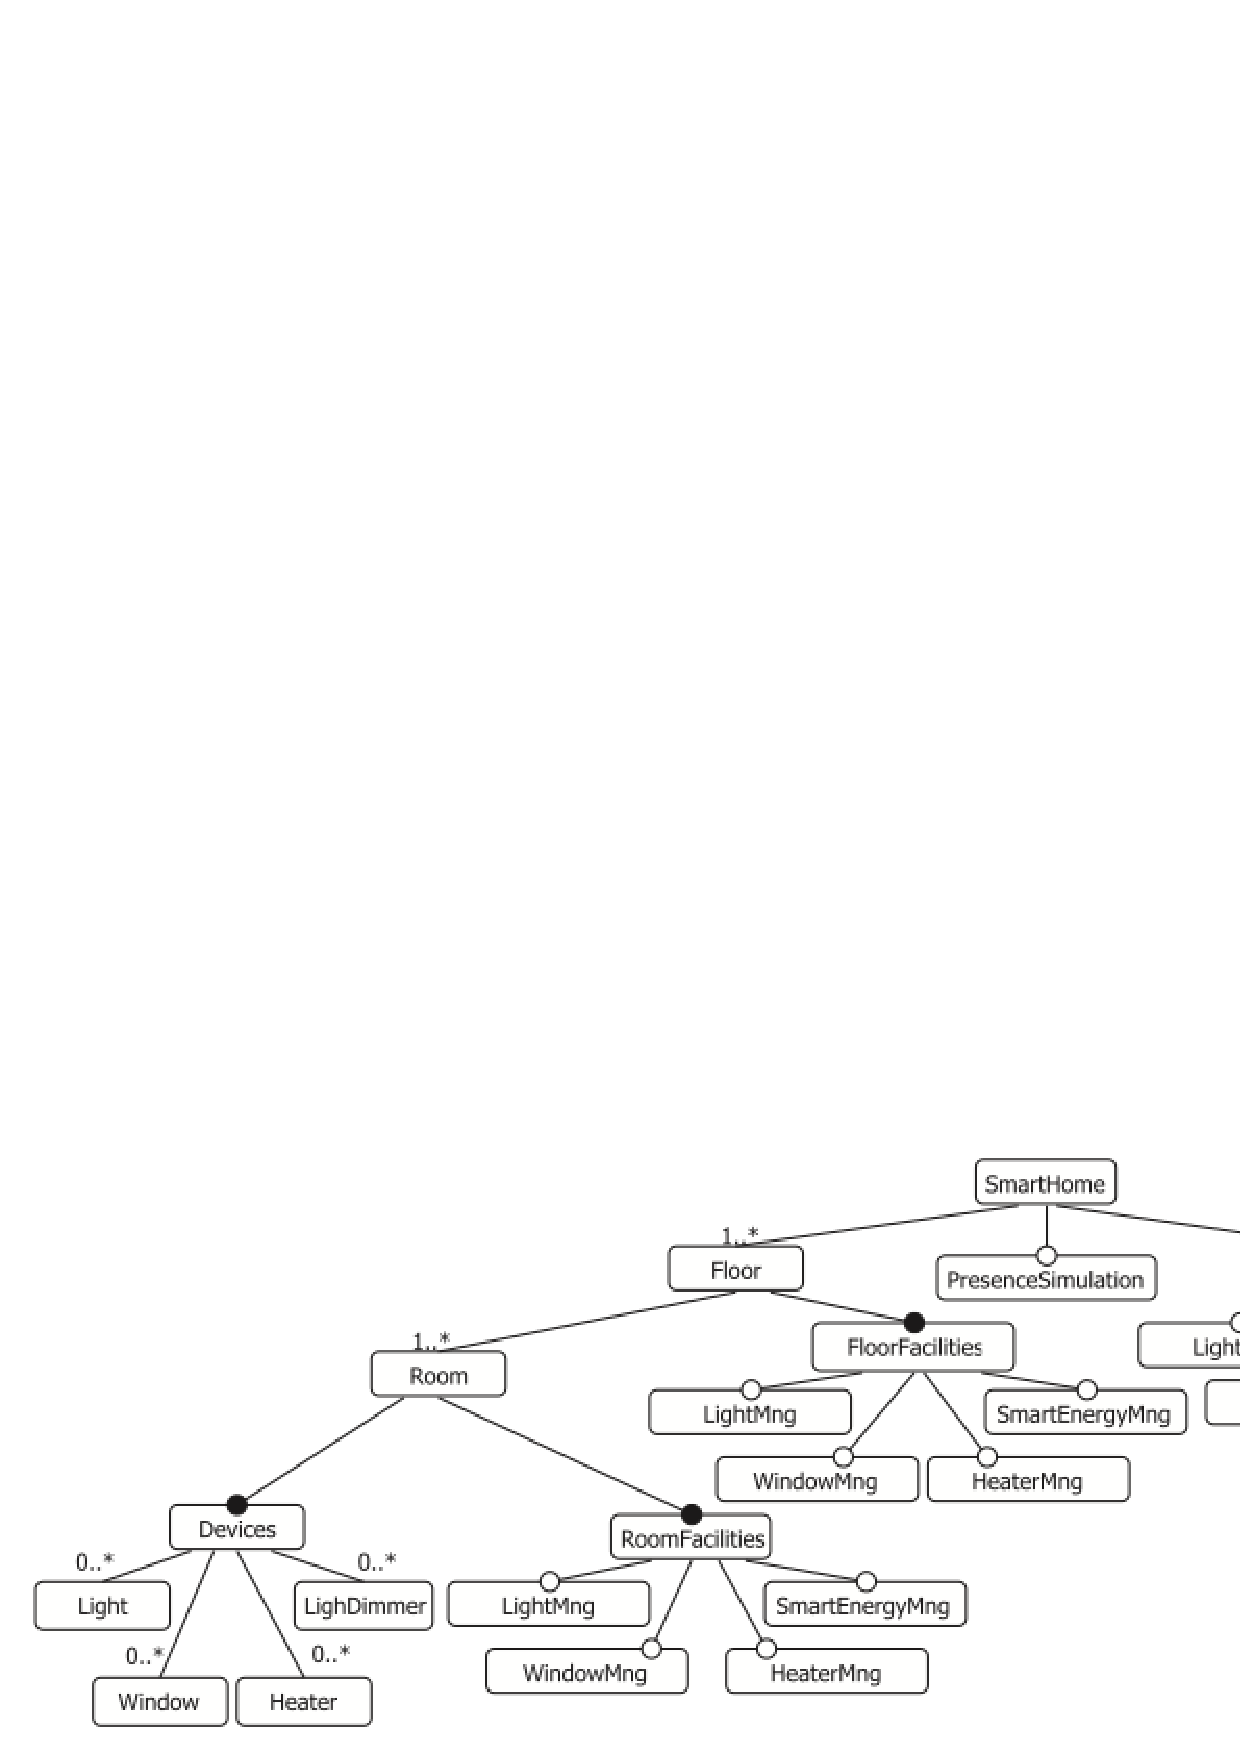
\includegraphics[scale=0.5]{background/featuremodel.jpg}
\caption{�rbol de caracter�sticas para crear una SmartHome }
\label{fig7}
\end{figure}

La figura \ref{fig7} muestra un ejemplo de modelo de caracter�sticas. En este caso se trata de un modelo de una casa inteligente o SmartHome, a trav�s del cual, seleccionando ciertas caracter�sticas u otras podremos construir qu� tipo de casa queremos. Cada una de las m�ltiples casas diferentes que podamos construir es lo que se denonima una especializaci�n o configuraci�n de nuestro modelo de caracter�sticas.

El proceso de crear una configuraci�n a partir de un modelo de caracter�sticas se conoce como proceso de configuraci�n o proceso de especializaci�n. Consiste en transformar un modelo de caracter�sticas de tal forma que el modelo resultante sea un subconjunto de las posibles configuraciones denotadas por el primer modelo. La figura \ref{fig8} muestra una posible configuraci�n para el modelo de caracter�sticas de la figura \ref{fig7}.

\begin{figure}[t]
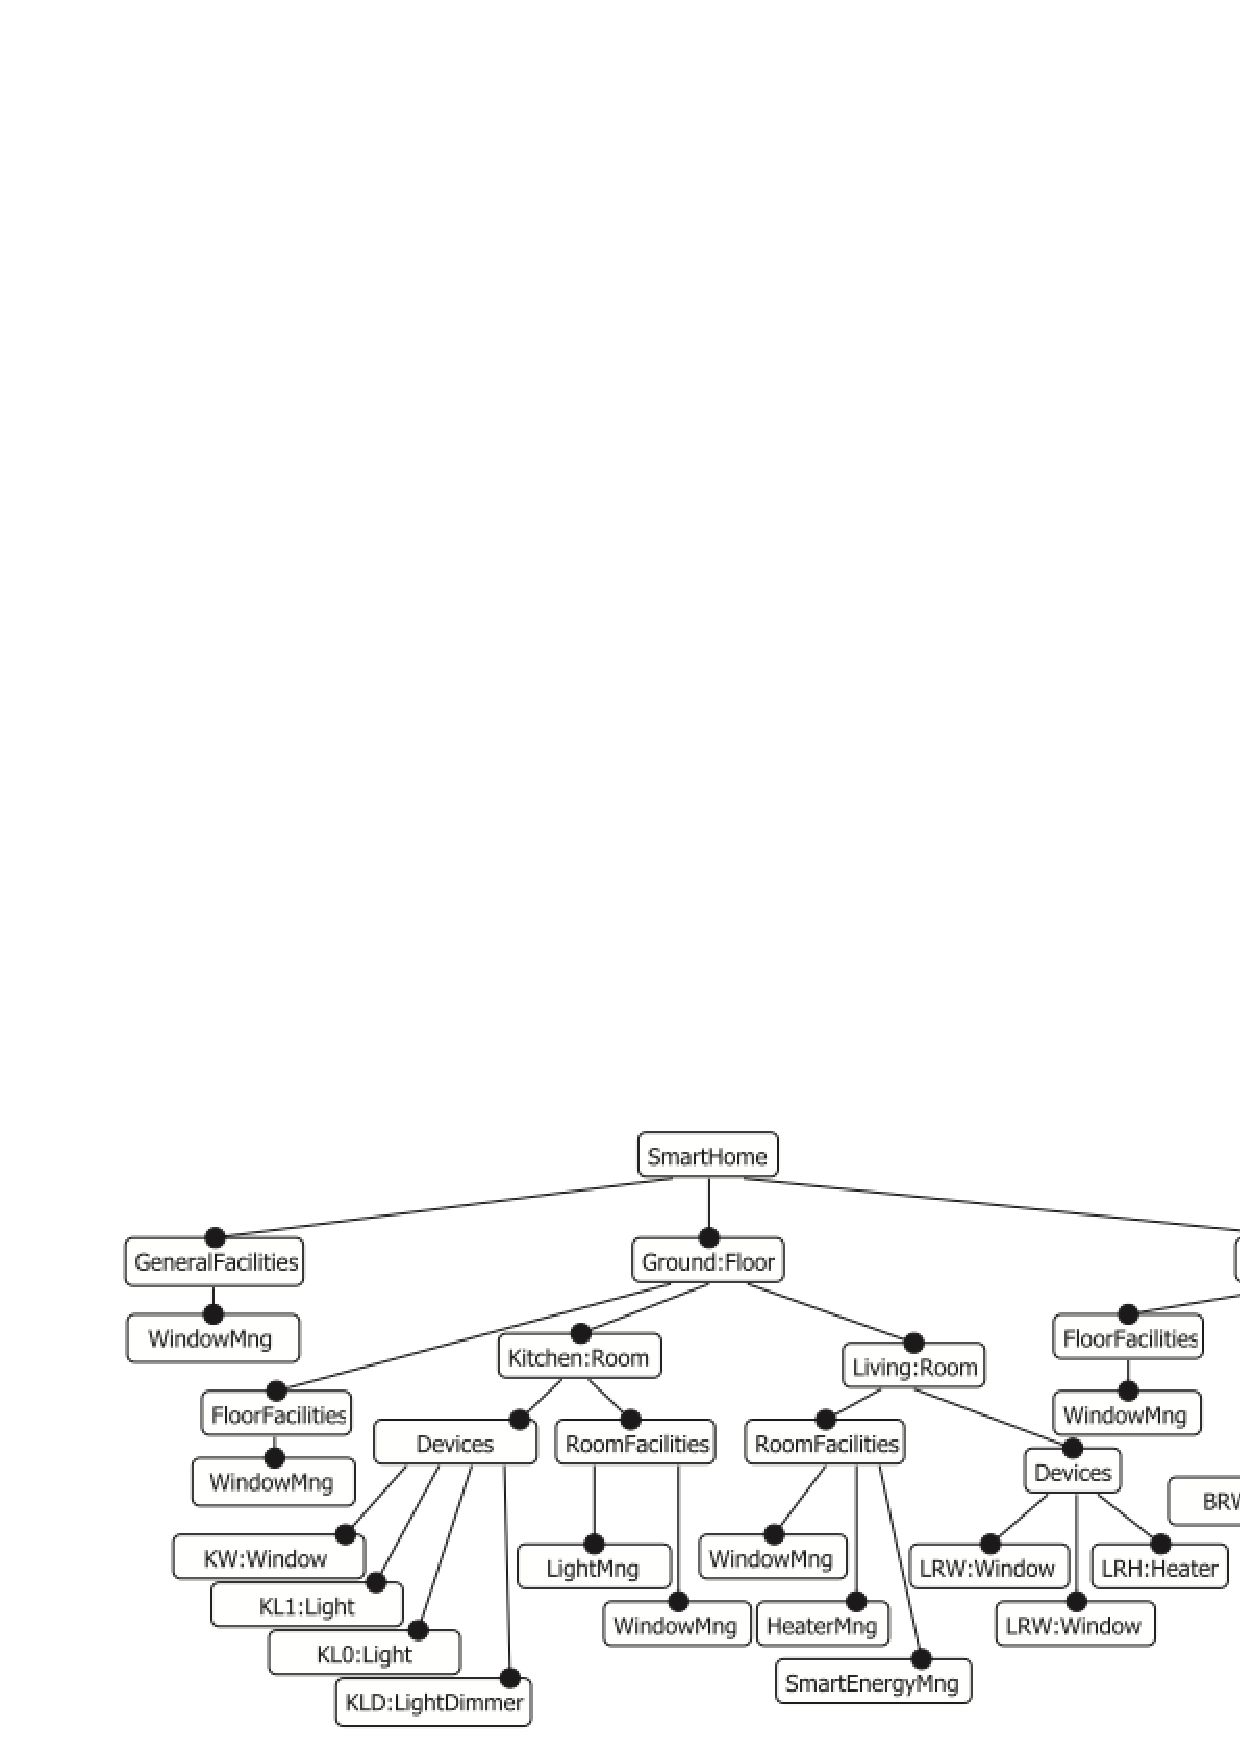
\includegraphics[scale=0.5]{background/configuration.jpg}
\caption{Especializaci�n del modelo de la figura \ref{fig7}, que representa una de las posibles casas que se pueden construir }
\label{fig8}
\end{figure}

La relaci�n entre un diagrama de caracter�sticas y una configuraci�n es an�loga a la existente entre una clase y una de sus instancias en programaci�n orientada a objetos.







\section{Arquitectura de plugins de Eclipse}
\label{sec:back:eplugins}
%%==================================================================%%
%% Author : Tejedo Gonz�lez, Daniel                                 %%
%%          S�nchez Barreiro, Pablo                                 %%
%% Version: 1.0, 18/11/2012                                         %%                   
%% Version: 1.0, 06/02/2013                                         %%                   
%%                                                                  %%
%% Memoria del Proyecto Fin de Carrera                              %%
%% Antecedentes, arquitectura de plugins de eclipse                 %%
%%==================================================================%%

En entorno de desarrollo Eclipse es un ejemplo de arquitectura modular f�cilmente extensible mediante una compleja, pero sencilla al programador, arquitectura de \emph{plug-ins}. Un \emph{plug-in} en Eclipse es un componente que provee un cierto tipo de servicio dentro del contexto del espacio de trabajo de Eclipse. Es decir, una herramienta que se puede integrar en el entorno Eclipse junto con sus otras funcionalidades. Dado que la herramienta \emph{Hydra} fue dise�ada como un \emph{plug-in} para Eclipse, y nuestro editor pretende integrarse tanto en \emph{Hydra} como en \emph{Eclipse}, es necesario conocer y manejar el funcionamiento de la arquitectura de plug-ins de Eclipse.

%%==============================================================================================%%
%% NOTA(Pablo): Esto no se entiende nada
%%==============================================================================================%%
%%
%% En particular, se han utilizado mucho los puntos de extensi�n. Un punto de extensi�n en un
%% plug-in indica la posibilidad de que ese plug-in sea a su vez parte de otro, o que haya 
%% otros plug-ins que sean parte de �l. Esta particularidad permite no s�lo la integraci�n de 
%% nuestro editor con Hydra, sino tambi�n la personalizaci�n de men�s y botones para �l 
%% gracias a la creaci�n de puntos de extensi�n con plug-ins de creaci�n de men�s y barras de
%% herramientas.
%%
%%==============================================================================================%%

%%==============================================================================================%%
%% NOTA(Pablo): Para solucionar
%% - Describir en uno o dos p�rrafos c�mo funciona la arquietctura de plug-ins para Eclipse
%% - Poner un ejemplo de punto de extensi�n, sencillo y concreto, y explicar como funciona 
%%   el punto de extensi�n utilizando algo de c�digo.
%% Si no sabes como escribir esta secci�n, la eliminas directamente, y actualizas la intro 
%% al Cap�tulo de forma conveniente.
%%==============================================================================================%%
